% 1110(본책 154쪽) — 세 지점 A, B, C 를 잇는 길(A–B 2개 · B–C 3개 · A–C 직행 1개). 스캔 삽화라 TikZ 로 다시 그림. 라벨은 원문 그대로 A, B, C 만.
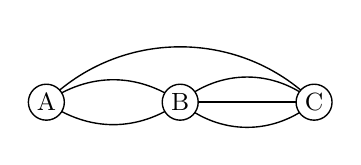
\begin{tikzpicture}[line width=0.5pt, font=\small]
  \coordinate (A) at (0,0); \coordinate (B) at (1.7,0); \coordinate (C) at (3.4,0);
  \draw (A) to[bend left=35] (B);
  \draw (A) to[bend right=35] (B);
  \draw (B) to[bend left=40] (C);
  \draw (B) -- (C);
  \draw (B) to[bend right=40] (C);
  \draw (A) to[bend left=45] (C);
  \node[circle, draw, fill=white, inner sep=1pt, minimum size=13pt] at (A) {$\mathrm{A}$};
  \node[circle, draw, fill=white, inner sep=1pt, minimum size=13pt] at (B) {$\mathrm{B}$};
  \node[circle, draw, fill=white, inner sep=1pt, minimum size=13pt] at (C) {$\mathrm{C}$};
\end{tikzpicture}
